\documentclass[conference]{IEEEtran}
\usepackage{blindtext, graphicx}
\usepackage[spanish]{babel}
\usepackage{skmath}
\usepackage[utf8]{inputenc}
\usepackage{amsmath}
\usepackage{amsfonts}
\usepackage{graphicx}
\usepackage[colorinlistoftodos]{todonotes}
\usepackage{algorithm}
\usepackage{algpseudocode}
\documentclass[conference]{IEEEtran}
\usepackage{blindtext, graphicx}
\usepackage[spanish]{babel}
\usepackage{skmath}
\usepackage[utf8]{inputenc}
\usepackage{amsmath}
\usepackage{amsfonts}
\usepackage{graphicx}
\usepackage[colorinlistoftodos]{todonotes}
\usepackage{algorithm}
\usepackage{algpseudocode}
\usepackage{pgfplots}
\pgfplotsset{width=9cm,compat=1.9}
\graphicspath{ {C:/Users/CASA/Pictures} }

\begin{document}
\title{$II$ Segundo Proyecto Programado Backtracking}
\author{\IEEEauthorblockN{Daniel Alvarado Bonilla}
\IEEEauthorblockA{Instituto Tecnol\'ogico de Costa Rica\\Ingenier\'ia en Computaci\'on\\
2014089192\\
Email: daniel.alvarado.bonilla@gmail.com}
\and
\IEEEauthorblockN{Roberto Rojas Segnini}
\IEEEauthorblockA{Instituto Tecnol\'ogico de Costa Rica\\Ingenier\'ia en Computaci\'on\\
2016139072\\
Email:rojassegniniroberto@gmail.com}
}
\maketitle
\begin{abstract}
%\boldmath
%\blindtext[1]
ACA VA EL ABSTRACT
\end{abstract}
\begin{IEEEkeywords}
O Grande, Matriz, Algoritmo.
\end{IEEEkeywords}
\section{Introducci\'on}
Existen much\'isimos tipos de algoritmos y un programador se define en cual tipo de algoritmo se escoge para resolver un determinado problema que tiene una variedad soluciones. Se debe entender el por qu\'e de la escogencia de este tipo. Es decir, en ocaciones no se quiere utilizar el algoritmo mas eficiente, esto no quiere decir que se tiene que utilizar un algoritmo mal fundamento, si no todo lo contrario, poder saber cuando se debe hacer uso de un algoritmo que no se basa en su eficiencia.\\
Un o de estos tipos de algoritmos es llamado Backtracking o "Vuelta Atras". Este algoritmo se basa en construir soluciones parciales a medida que se progresa en el arbol de opciones de nuestro problema.  En otras palabras es una t\'ecnica de programaci\'on para hacer una b\'usqueda sistem\'atica a tra\'aves de todas las posibles configuraciones de nuestro problema. Todos los algoritmos de backtracking siguen un mismo patr\'on, pero var\'ia un poco con el problema. \\Se puede observar su forma gen\'erica en la secci\'on de Pseudoc\'odigos.
\\
En el presente trabajo se investigo, trabajo para crear una pequeña aplicaci\'on con el fin de que este genere Kakuros.  Un kakuro es un enigma l\'ogico que es semejante al conocido Crucigrama. Pero este no usa letras ni palabras, si no, n\'umeros. Se les conoce tambi\'en como Suma Cruzada, es un juego bastante popular en Jap\'on. 
El algoritmo de backtracking explicado anteriormente es utilizado para resolver diferentes Kakuros. Para mejor la eficiencia del mismo, se inventaron diferentes algoritmos mas pequeños de "poda" para asi disminuir de manera significante el \'arbol de posibles soluciones.  Para las diferentes funciones se hizo un an\'alisis de O grande y se realizaron distintos experimentos.
\begin{figure}
	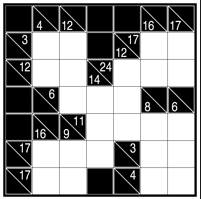
\includegraphics[scale=0.5]{kakuroImg.png}
	\caption{Kakuro}
\end{figure}
\section{Pseudoc\'odigo}
  \begin{algorithm}
   \caption{Backtracking  Generic Algorithm}
    \begin{algorithmic}[1]
      \Function{backTracking}{$v[1..k]$ }\\\Comment{v es un vector $k$prometedor}
		\\
        \State si v es una solucion entonces escribir v
        \For{ para cada vector$(k+1)-$prometedor w}
        \State tal que $w[1..k] = v[1..k]$
        \State hacer backTracking$(w[1..k+1])$
        \EndFor
       \EndFunction
\end{algorithmic}
\end{algorithm}

  \begin{algorithm}
   \caption{Solve - Backtracking Algorithm implemented}
    \begin{algorithmic}[1]
      \Function{solveKakuro}{$kakuro$ }\\\Comment{kakuro es una matriz, la cual contiene el kakuro sin soluci\'on}
		\\
		\If{noEmptySpaces(kakuro)}:
		    \If{isKakuroSolved(kakuro)}:
		        \State return True
		    \Else{}:
		        \State return False
		 \Else{}
		    \State position=getNextPosition(kakuro)
		    \State row=position[0]
		    \State column=position[1]
		    \State num1 = getNumberLeft(kakuro, position)
		    
		    \If{num1 == 0}:
		        \State num1 = -25
		    \EndIf
		    \State num2 = getNumberUp(kakuro, position)
		    
		    \If{num2 == 0}:
		        \State num2 = -25
		    \EndIf
		    
		    \State deleteRepeatedValues(kakuro,getIntersection
		    \State (getValues(kakuro,position,num1,num2),
		    \State getValuesList(num1,num2,kakuro,position)),position)
		    
		    \If{values==[]}:
		        \State return False
		    \EndIf
		    
		    \For{i en el largo de values}
		        \State value = values[i]
		        \State kakuro[row][column] = value
		        \If{solveKakuro(kakuro)}:
		            \State return True
		        \Else{}:
		            \State kakuro[row][column] = BLANK\_ SPACE
		    \EndFor
		    
	\State return False

       \EndFunction
\end{algorithmic}
\end{algorithm}





  \begin{algorithm}
   \caption{substract Values Algorithm}
    \begin{algorithmic}[1]
      \Function{substractVal}{$k[1..k]$,$p[x,y] $,$sum$,$bool$ }\
        \State newSum = 0
        \State newSpaces = 0
        \If{left}
        		\State row = p[0]
        		\State col = p[1]
        		\While{col$ >= 0$}
        			\If{k[row][col] es vector}
        				\State spaces = getSpaces()
        				\State break
        			\EndIf
        			\State col$-$
        		\EndWhile
        		\State col $+ 1$
        	\EndIf
        	\For{i en rango de spaces}
        	\If{k[row][col$+i$]  tiene un valor entonces}
        		\State spaces $-= 1$
        		\State sum $-= $ [el valor que este en esa posici\'on]
        	\EndIf
        	\EndFor
        	\If{not left}
        		\State row = p[0]
        		\State col = p[1]
        		\While{col$ >= 0$}
        			\If{k[row][col] es vector}
        				\State spaces = getSpaces()
        				\State break
        			\EndIf
        			\State row$- 1$
        		\EndWhile
        		\State row $+ 1$
        	\EndIf
        	\For{i en rango de spaces}
        	\If{k[row$+i$][col]  tiene un valor entonces}
        		\State spaces $-= 1$
        		\State sum $-= $ [el valor que este en esa posici\'on]
        	\EndIf
        	\EndFor \\
		\Return sum,spaces
       \EndFunction
\end{algorithmic}
\end{algorithm}

  \begin{algorithm}
   \caption{Get Values Algorithm }
    \begin{algorithmic}[1]
      \Function{getValuesList}{$hSum$ $vSum$,$k[1..k]$,$p[x,y] $ }\
      \State  sumUp,spacesUp = substractValues(k,p,vSum,False)
      \State  sumLeft,spacesLeft = substractValues(k,p,hSum,True)
      \If{si el valor forma una suma vertical}
     	 	\If{spacesUp = 1}
     	 			\If{Si es una intersecci\'on de dos sumas}
     	 				\Return [sumUp]
     	 			\EndIf
     	 	\If{spacesLeft =1}
     	 			\If{si ambas sumas son iguales}
     	 					\State \Return [sum]
     	 			\Else
     	 			 		\State \Return vac\'io
     	 			\EndIf
     	 	\Else
     	 			\State combinaciones = getCombinations()
     	 			\Comment retorna un vector de combinacinoes que vienen de un diccionario	
     	 			\If{sumUp esta en combinaciones}
     	 					\State \Return [min de sumLeft y sumUp] si no []
     	 			\EndIf
     	 	\EndIf
     	 \Else
     	 		\State combinaciones = getCombinations()
     	 		\For{por combinacion en combinaciones]}
     	 			\State Agregar cada valor a un 
     	 			\State vector llamado valoresUp
     	 		\EndFor
     	 \EndIf
     \If{el valor forma una suma horizontal}
          	 	\If{SpacesLeft = 1}
     	 			\If{Si es una intersecci\'on de dos sumas}
     	 				\Return [sumLeft]
     	 			\EndIf
     	 	\If{SpacesUp =1}
     	 			\If{si ambas sumas son iguales}
     	 					\State \Return [sum]
     	 			\Else
     	 			 		\State \Return vac\'io
     	 			\EndIf
     	 	\Else
     	 			\State combinaciones = getCombinations()
     	 			\Comment retorna un vector de combinacinoes que vienen de un diccionario	
     	 			\If{sumUp esta en combinaciones}
     	 					\State \Return [min de sumLeft y sumUp] si no []
     	 			\EndIf
     	 	\EndIf
     	 \Else
     	 		\State combinaciones = getCombinations()
     	 		\For{por combinacion en combinaciones]}
     	 			\State Agregar cada valor a un 
     	 			\State vector llamado valoresLeft
     	 		\EndFor
     	 \EndIf
     	 \EndIf
      \EndIf
      \State \Return intersecci\'on entre valoresLeft y valoresRight
       \EndFunction
\end{algorithmic}
\end{algorithm}




\begin{algorithm}
   \caption{Repeated Number Algorithm }
    \begin{algorithmic}[1]
      \Function{numberRepeated}{$num$,$k[1..k]$,$p[x,y] $ }\
      \State row = p[0]
      \State col = p[1]
      \While{el espacio sea diferente de vacio o la longitud }
      	\If{si el numero que hay en la posicion es igual al valor recibido}
      		\State\Return  True
      	\EndIf
      	\State Pasar a la siguiente posici\'on
      \EndWhile
      \State \Return False 
       \EndFunction
\end{algorithmic}
\end{algorithm}



\section{Complejidad de los Algoritmos}

\subsection{Orden de $O(f(n))$ de Función de Poda}:\\
Este algoritmo tiene en s\'i bastantes funciones  pequeñas. Cada una siendo fundamental para la funci\'on de poda. Las m\'as relevantes se explicar\'an a continuaci\'on son:\\
\begin{enumerate}[I]
\item SubstractVal() es una funci\'on que toma el lugar donde se puede colocar un valor$[1..9]$, recibe tambi\'en este valor que se utilizar\'a las sumas a las que pertenece, el mejor caso es que sea una intersecci\'on de dos sumas, asi la lista de valores seria menor. Toma esta posici\'on y se mueve ya sea de forma vertical u horizontal, hasta buscar la suma a la que pertenece esa posici\'on. Al encontrar el vector $v[sumaVertical,sumaHorizontal]$ se desplaza contando los espacios disponibles que tiene esta suma.  Esto es un comportamiento lineal, es decir $O(n)$ al recorrer una lista. Lo interesante de este algoritmo es que una vez obtenida la cantidad de espacios, se recorre de nuevo desde la posici\'on en la que se encuentra el vector v mencionado anteriormente, y suma los las casillas que ya tienen  un valor. Y por cada casilla que tenga un valor, se aumenta un contador llamado newSpaces. Este es otro comportamiento lineal, es decir hasta el momento es un $O(2n)$. Este paso es sumamente importante, por que resta a la suma que se tiene que llegar, lo que se tiene hasta el momento. En otras palabras, si se debe llegar a sumar un total de $27$ en cuatro espacios, y ya se tiene $2$ espacios utilizados, se toman los valores de estos dos espacios, se suman y luego se le restan al $27$. Si se ten\'ia $3$ y $7$ la nueva suma a la que se tiene que llegar es $17$. Por \'ultimo este numero y los espacios nuevos  $(2)$ son retornados. Hasta el momento se tiene $O(2n)$. \\
Ver Algoritmo 3. 
\item La funci\'on getValuesList es aquella que interpreta los valores retornados por substractVal(). Este primero revisa si dicha posici\'on donde se colocar\'a el valor es intersecci\'on de una suma en forma vertical y/o forma horizontal. Si pertenece a alguna de las anteriores, se verifica si tiene y si solo un espacio disponible, se utiliza una pequeña funcion la cu\'al retorna de un diccionario creado, donde este de llaves la cantidad de espacios disponibles, para cada de estas llaves tiene una llave secundaria la cual es la suma que puede formarse. Por \'ultimo, tiene un vector de vectores con las posibles combinaciones de valores para obtener esta suma en dicha cantidad de espacios.  Al obtenerla, se verifica que la suma, la cual es el unico valor que puede colocarse en la posici\'on dada, si no esta en estas combinaciones, se hace backtracking. Retorna una lista vac\'ia, donde el algoritmo principal ve que no tiene opciones que utilizar y se devuelve. Si la cantidad de espacios es diferente a uno, usando la funci\'on que obtiene las combinaciones, se agregan todos los valores posibles a una lista. Esto se hace para cada suma, siempre y cuando la posici\'on en la que se encuentra el algoritmo sea intersecci\'onTodo lo dicho anteriormente es de un orden lineal, sumando $O(2n + n)$. Esta funci\'on retorna este vector con los posibles valores que pueden ser utilizados y as\'i la funci\'on principal pruebe con estos.\\
Ver Algoritmo 4.

\\

\item  La funci\'on numberRepeated() tiene un comportamiento lineal. Esta funci\'on recibe un valor y toma una desici\'on. Se mueve de forma horizontal y vertical, lo cual es recorrer un vector, buscando todos los numeros que tiene y comparandolos con el valor recibido. Si el valor esta repetido, la funci\'on retorna True. La O grande de esta pequeña funci\'on es $O(n)$,
El orden de la funci\'on de poda es de $O(n)$ ya que $3$ es una constante que no afecta el comportamiento de dicha funci\'on.\\



\end{enumerate}
El orden de la funci\'on de poda es de $O(n)$ ya que $3$ es una constante que no afecta el comportamiento de dicha funci\'on.


\newline

\newline




\subsection{Orden de $O(f(n))$ de Permutaciones:}\\
Para resolver el problema no se utilizo un algoritmo espec\'ifico que obtuviese todas las permutaciones. Lo implementado fue, ir rellenando espacio por espacio un n\'umero a la vez. La funci\'on de la poda, analiza y obtiene los posibles valores que pueden colocarse en cada espacio en blanco. Y para la lista total de valores, coloca ese valor en dicha posici\'on y llama a la funci\'on principal de backtracking con solo un campo m\'as resuelto. Donde el valor utilizado es prometedor hasta llegar a un punto donde la funci\'on de poda determina que para ese lugar con los numeros y espacios que existen hasta el momento ya no hayan opciones, esto resultando a hacer backtrack. Dicho lo anterior se considera que el algoritmo de permutar es una constante, donde puede basarse en una lista de numeros que debe recorrerse nunca mayor a una longitud de nueve.
\newline


\subsection{Orden de $O(f(n))$ de Backtracking}
El algoritmo de Backtracking implementado se deduce que tiene un orden $O(n^k)$. $N$ es la cantidad de opciones que pueden colocarse en un determinado espacio del Kakuro. Al ser un \'arbol de soluciones, $N$ el nivel del nodo,  donde cada nodo tiene sus propios nodos, esto implica $n(n-1)(n-2)...(n-k+1)$. O grande considera el peor de los casos y este seria recorrer cada nodo hasta su ultimo nivel, es decir recorrer el \'arbol a profundidad. Siendo un comportamiento de $n^k$. Existe una funci\'on la cual recorre la matriz del Kakuro para encontrar una posici\'on libre, esta parte es $O(n^2)$. En total, $O(n^k + n^2)$ pero al como O Grande utiliza el peor de los casos, se concluye $O(n^k)$



\section{Experimentos}
\subsection{Experimento 1: hilos}

    La utilización de hilos es ampliamente utilizada para mejorar el tiempo de ejecución de programas y algoritmos. Es posible ejecutar programas (o pedazos de ellos) de manera concurrente, en algunos casos, y de manera paralela, en otros, mediante la utilización de hilos.\newline
    
    Un hilo ejecuta cierto pedazo de código de un programa de manera "separada" y permite realizar múltiples operaciones casi simultáneamente. Muchas veces, las capacidades del sistema en el que se corre el programa (computadora), las características del lenguaje de programación utilizado y algunos otros aspectos dictan la manera en el que los hilos serán ejecutados.\newline
    
    En el caso pertinente a este proyecto, se implementaron hilos utilizando la librería \textbf{threading} de Python. Dicha librería permite crear y ejecutar hilos de manera fácil y sencilla, utilizando la función \textbf{Thread}.\newline
    
    Python es capaz de ejecutar hilos de manera paralela. Sin embargo, la implementación utilizada de los mismos corresponde a una manera simple, ajena del uso de piscinas de hilos y otras características, la cual corre los hilos, muy probablemente, de manera concurrente.\newline
\subsection*{Hipótesis}

    A pesar de esto, es de esperar que la utilización de hilos mejore los tiempos de ejecución. Además, se tiene como hipótesis que conforme aumente la cantidad de hilos, el tiempo empeorará y el programa durará más ejecutándose.\newline

\subsection*{Metodología}

    Para probar (o refutar) la hipótesis, se ejecutó el programa 1000 veces, con el objetivo de resolver un kakuro determinado (ver Figura 2). Para cada ejecución se varió la cantidad de hilos máximos que se podían utilizar. Las cantidades de hilos utilzadas son: dos, cinco, ocho, quince, cincuenta, ciento cincuenta, trescientos, quinientos, setecientos cincuenta y mil. Se guardó el tiempo de ejecución en milisegundos.\newline
    

\subsection*{Resultados}

    Los resultados demostraron que aumentar la cantidad de hilos empeora el tiempo de ejecución del programa. A pesar de que los tiempos no mostraban un incremento constante (en algunas partes el tiempo fluctuaba), la tendencia se mantenía a la alta conforme la cantidad de hilos aumentaba. El uso de 150 hilos hizo que se duplicara el tiempo de ejecución (244.842 milisegundos en el caso base (sin hilos), 487.662 con 150 hilos). \newline 
    
        No se notó mejoría en los tiempos en ningún caso, en relación con la ejecución sin hilos. Las diferencias, sin embargo, entre el uso de 0 a 50 hilos fueron mínimas. \newline
        
        Entre los 350 y 750 hilos, el tiempo de ejecución sufrió una baja en los tiempos. De nuevo, estas diferencias son mínimas, pero demuestran que la utilización de hilos se ve sujeta a fluctuaciones de este tipo.
        
      
\subsection*{Gráficos y anexos}



\begin{tikzpicture}
\begin{axis}[
    title={Comparación de tiempos de ejecución  \newline utilizando y sin utilizar hilos},
    ylabel={Tiempo de ejecución (milisegundos)},
    xlabel={Cantidad de hilos},
    xmin=0, xmax=1000,
    ymin=0, ymax=600,
    xtick={},
    ytick={},
    legend pos=north west,
    ymajorgrids=true,
    grid style=dashed,
    width=9cm
]
 
\addplot[
    color=blue,
    mark=square,
    ]
    coordinates {
    (0, 244.842)(2,267.853)(5, 266.163)(8, 278.31)(15, 266.696)
    (50, 286.397)(150,487.662)(300, 502.992)(500, 502.339)(750, 496.937)
    (1000, 520.317)
    };
    %\legend{CuSO$_4\cdot$5H$_2$O}
 
\end{axis}
\end{tikzpicture}

\begin{figure}
	
\includegraphics[scale=0.3]{kakuroHardPhoto.png}
	\caption{Kakuro utilizado}
\end{figure}

\newpage
\subsection{Experimento 2: forks}

    Como se discutió anteriormente, los hilos permiten paralelizar procesos y código. Un hilo ejecuta cierto pedazo de código. Otra manera de paralelizar un proceso es por medio del uso de \textbf{forks}.\newline
    
    Un fork es un proceso que se ejecuta de manera independiente al proceso principal de un programa. El fork es una copia del proceso en el que fue llamado. Todas las variables, funciones y características del proceso padre son heredadas al proceso hijo.\newline
    
\subsection*{Hipótesis}

    Como con el experimento anterior, el objetivo de implementar forks es determinar si hay una reducción significativa en el tiempo de ejecución. Sin embargo, es de esperarse que muchos procesos corriendo al mismo tiempo empeoren los tiempos de ejecución. \newline
    
\subsection*{Metodología}

    Se ejecutó el programa con un total de cero, uno, dos, cinco y siete forks. Por cada valor de los mencionados, se corrió el programa diez veces y se extrajo un promedio de tiempo en milisegundos. El kakuro utilizado es el mismo que el del experimento anterior (ver Figura 2).


\subsection*{Resultados}

    Los forks resultaron ser mucho más pesados que los hilos. La generación de más de diez procesos simultáneos provocó que el programa corriera con dificultades. Después de ese punto, el programa por lo general se paralizaba y un reinicio de la computadora era necesario.\newline
    
    Como era de esperarse, el aumento de forks provocó un crecimiento sustancial del tiempo de ejecución. Entre el uso de dos y cinco forks, se observó un aumento de casi siete veces del tiempo. El mismo comportamiento se observó entre cinco y siete forks.\newline
    
    Aunque entre el uso de cero y un fork hubo una diferencia negativa en el promedio general (el tiempo aumentó al crear un fork), al analizar los tiempos individuales de las corridas se puede notar que, en algunos casos, el uso de un fork mejoró el tiempo de ejecución del programa. Es más, en la mayoría de las corridas el tiempo fue notablemente inferior. Sin embargo, el promedio general de las corridas con un fork, en el final, resultó ser mayor.\newline
    
    Más allá de la ventaja de usar un fork sobre prescindir de su uso, los forks presentaron un comportamiento inestable y de alto consumo computacional. Para un programa como el que corresponde a este proyecto (resolución de kakuros), los forks no presentaron una mejora significativa y las operaciones se vieron, en general, afectadas negativamente por el costo computacional de manejar los procesos simultáneamente. \newline
    

\subsection*{Gráficos y anexos}


\begin{tikzpicture}
\begin{axis}[
    title={Comparación de tiempos de ejecución  \newline utilizando y sin utilizar forks},
    ylabel={Tiempo de ejecución (milisegundos)},
    xlabel={Cantidad de hilos},
    xmin=0, xmax=10,
    ymin=0, ymax=27000,
    xtick={},
    ytick={},
    legend pos=north west,k
    ymajorgrids=true,
    grid style=dashed,
    width=9cm
]
 
\addplot[
    color=blue,
    mark=square,
    ]
    coordinates {
    (0, 498.433)(2, 513.2)(5, 6835.1)(7, 26547)
    };
    %\legend{CuSO$_4\cdot$5H$_2$O}
 
\end{axis}
\end{tikzpicture}




\subsection{Experimento 3: tamaños y tiempos}

    Como se determinó anteriormente, el orden del algoritmo de backtracking para resolver los kakuros es, en el peor de los casos, $n^k$. Un orden exponencial posee un comportamiento de constante crecimiento (en el caso de los algoritmos). Este crecimiento es acelerado y pronunciado.\newline
    
    ¿Se reflejará este comportamiento en la ejecución real del algoritmo? Es de esperarse que las tendencias temporales de las ejecuciones estén sujetas a la teoría. Sin embargo, diversos aspectos pueden influir para que el espacio teórico y el espacio real discrepen en temas de costo y ejecución de los algoritmos.\newline
    
    Además, es común que el tamaño de la entrada de un algoritmo determine el tiempo que durará ejecutándose. Un algoritmo con un comportamiento exponencial, durará más resolviendo un problema entre mayor sea la entrada. Lo anterior es cierto para algoritmos que trabajan con imágenes, por ejemplo, los cuales normalmente poseen una complejidad de $n^2$: entre más grande sea la imagen, más se tardará en recorrerla y ejecutar el algoritmo.\newline
    
    Los kakuros se parecen a las imágenes: son matrices (en este caso cuadradas) que contienen valores en cada una de sus casillas. ¿Se comportarán de manera similar? A primera instancia, es justo suponer que el tiempo necesario para resolver un kakuro debería incrementar según el tamaño del mismo. ¿Es esto cierto? Los resultados del experimento demuestran que no.\newline
    
    
    
\subsection*{Metodología}

    Para comprobar la hipótesis planteada, se ejecutó el algoritmo de resolución de kakuros en tres puzles diferentes, con tamaños distintos: de cinco por cinco; de diez por diez; dos de veinte por veinte y de treinta por treinta.\newline
    
\subsection*{Resultados}

    Los resultados fueron los siguientes (tiempos de ejecución dados en milisegundos): para el kakuro 5x5, 0.058; para el 10x10, 509.745; para el primero 20x20, 218.498; para el segundo 20x20, 277.822.\newline
    
    Los resultados del experimento muestran que los dos kakuros de mayor tamaño fueron resueltos en la mitad del tiempo que el kakuro de 10x10. Es decir, la mitad del tiempo para el doble de tamaño.\newline
    
    Lo evidenciado por los experimentos se debe al hecho de que la complejidad del algoritmo para los kakuros no depende directamente del tamaño del kakuro. En lugar de esto, la complejidad de ve influenciada por la cantidad de casillas que pueden albergar números, las sumas, las intersecciones, la cantidad de permutaciones que puede poseer un conjunto de casillas, la cantidad de soluciones posibles, entre otros factores.\newline
    

    
\subsection*{Gráficos y anexos}


\begin{tikzpicture}
\begin{axis}[
    title={Comparación de tiempos de ejecución  y tamaños},
    ylabel={Tiempo de ejecución (milisegundos)},
    xlabel={Tamaño del kakuro},
    xmin=0, xmax=30,
    ymin=0, ymax=600,
    xtick={},
    ytick={},
    legend pos=north west,k
    ymajorgrids=true,
    grid style=dashed,
    width=9cm
]
 
\addplot[
    color=blue,
    mark=square,
    ]
    coordinates {
    (5, 0.058)(10, 509.745)(20, 218.498)
    };
    %\legend{CuSO$_4\cdot$5H$_2$O}
 
\end{axis}
\end{tikzpicture}


    El gráfico anterior contrasta con la representación gráfica de una función exponencial (ver Figura 3). Solamente con el tamaño del kakuro no se puede predecir el comportamiento que el algoritmo tendrá ni el tiempo de ejecución. Un cálculo basado solamente en el tamaño del puzle difiere de la proyección teórica sobre el comportamiento del algoritmo. En palabras sencillas, la dificultad de un kakuro no se ve directamente afectada por el tamaño del mismo. 

\begin{figure}
	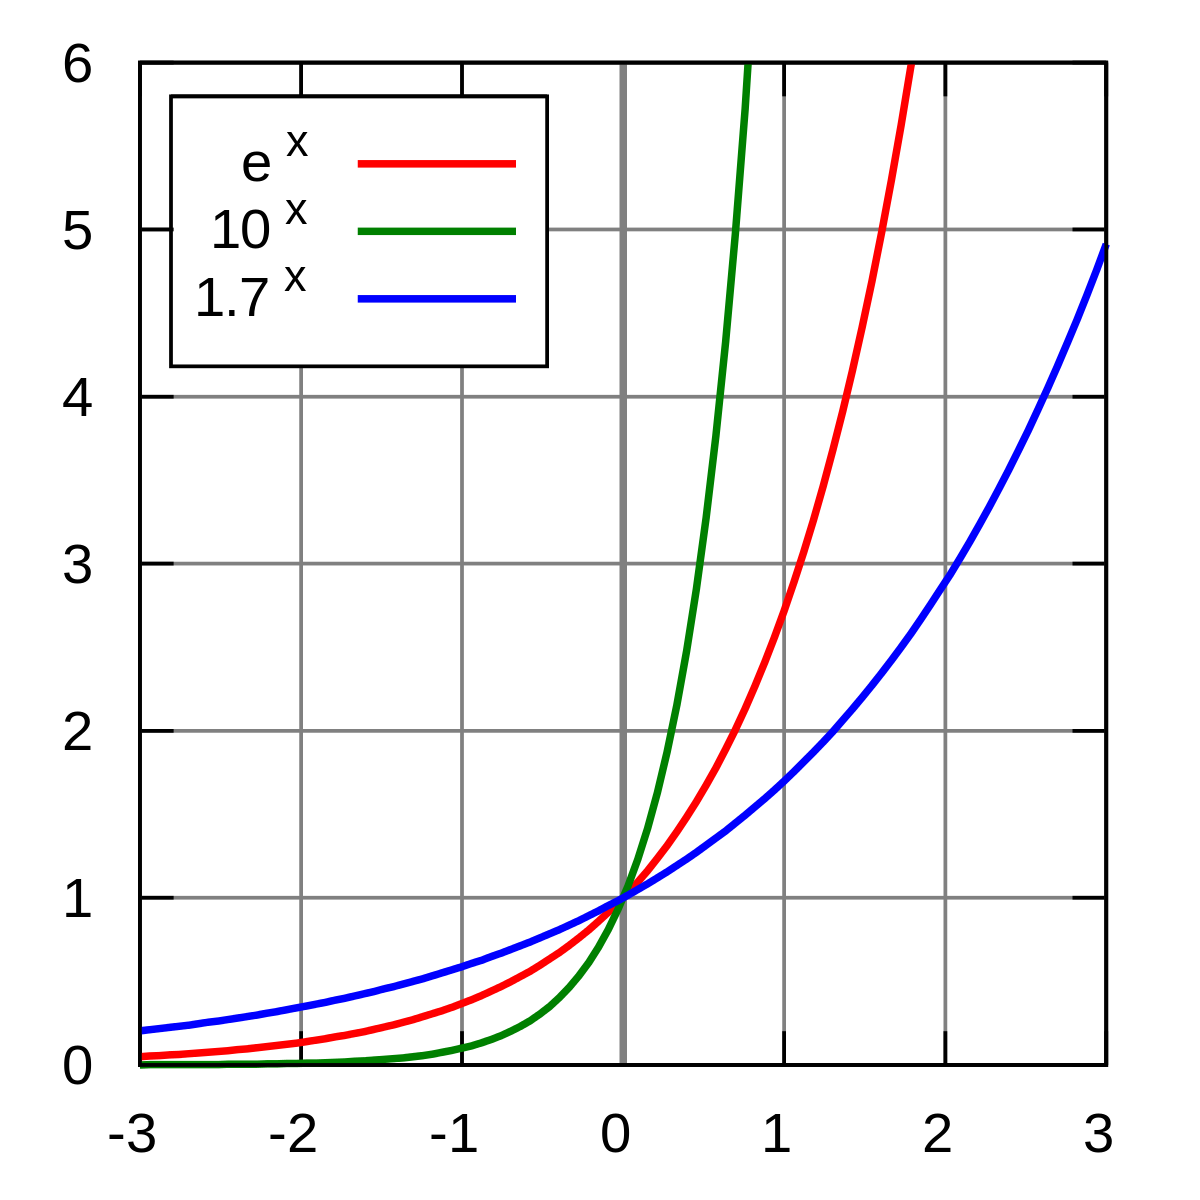
\includegraphics[scale=0.2]{exponencial.png}
	\caption{Ejemplo de funciones exponenciales}
\end{figure}


\subsection{Discusión}

\subsection*{Sobre hilos}
    Es interesante notar que el uso de hilos, en los experimentos realizados, no mejoró el tiempo de ejecución del programa. Es posible que lo anterior se deba a la implementación misma de los hilos. Existen diversas manera de implementar y manejar los hilos en un programa. En este proyecto, se utilizaron hilos "sencillos", cuya creación se realiza en una línea de código, mediante el uso de la librería \textbf{threading} de Python. Los hilos son creados en un ciclo y, después de eso, su ejecución es, de cierto modo, libre.\newline
    
    Existen otros métodos disponibles para implementar  hilos. Uno de ellos consiste en utilizar una piscina de hilos (del inglés \textit{thread pool}), la cual crea una estructura en la que los hilos (también llamados \textit{workers}) esperan recibir una orden de ejecución. De esta piscina salen los hilos que se ejecutan en el programa. El objetivo de la piscina es mejorar la concurrencia de procesos. Es posible que una implementación de este tipo genere mejores resultados en la resolución de los kakuros. Lo anterior, sin embargo, se escapa del alcance de este proyecto y queda para futuras revisiones y versiones del programa el utilizar hilos de esa manera.\newline



    


\begin{thebibliography}{1}

\bibitem{IEEEhowto:kopka}
H.~Kopka and P.~W. Daly, \emph{A Guide to \LaTeX}, 3rd~ed.\hskip 1em plus
  0.5em minus 0.4em\relax Harlow, England: Addison-Wesley, 1999.

\end{thebibliography}


\end{document}
